\section{模型结果}

\NewDocumentCommand\MyCompare{m m m}{($#1$\ vs.\ $#2$, $p<#3$)}

\subsection{基准特征}

从eICU数据库中提取出$100,308$条数据,包含$17,729$名不同的脓毒症患者。%
其中,$3,866\,(3.85\%)$条数据为正例,$96,442\,(96.15\%)$条数据为反例。

经过比较,正例数据拥有更长的ICU入住天数\MyCompare{21.067}{10.852}{0.001},%
更少的血浆蛋白\MyCompare{2.109}{2.520}{0.001},%
更少的淋巴细胞数目\MyCompare{9.931}{12.473}{0.001},%
更高的心率\MyCompare{93.337}{88.458}{0.001},%
更高的呼吸频率\MyCompare{21.814}{21.019}{0.001},%
更少的血清总蛋白\MyCompare{5.578}{5.928}{0.001},%
更低的红细胞比容\MyCompare{27.808}{29.888}{0.001},%
更少的肌酸酐\MyCompare{1.489}{1.610}{0.001},%
更高的白细胞计数\MyCompare{13.218}{12.189}{0.001},%
更多的血小板\MyCompare{260.259}{226.342}{0.001},%
更低的平均动脉压\MyCompare{79.727}{82.055}{0.001}。

\subsection{模型比较}

\begin{table}[htb]
    \centering
    \scriptsize
    \begin{threeparttable}
        \begin{tabular}{clcc}
            \toprule
            排名 & 模型名称                         & 平均准确率               & 平均AUC\tnote{1}      \\
            \midrule
            1  & CatBoost                     & $0.996 (\pm 0.001)$ & $0.996 (\pm 0.001)$ \\
            2  & Light Gradient Boosting      & $0.995 (\pm 0.001)$ & $0.996 (\pm 0.001)$ \\
            3  & Extreme Gradient Boosting    & $0.995 (\pm 0.001)$ & $0.994 (\pm 0.002)$ \\
            4  & Hist Gradient Boosting       & $0.994 (\pm 0.002)$ & $0.996 (\pm 0.002)$ \\
            5  & Ada Boost                    & $0.993 (\pm 0.002)$ & $0.995 (\pm 0.002)$ \\
            6  & Decision Tree                & $0.989 (\pm 0.002)$ & $0.949 (\pm 0.013)$ \\
            7  & Multi-Layer Perceptron       & $0.982 (\pm 0.004)$ & $0.975 (\pm 0.008)$ \\
            8  & SVM (RBF Kernel)             & $0.973 (\pm 0.003)$ & $0.957 (\pm 0.011)$ \\
            9  & Logistic                     & $0.966 (\pm 0.007)$ & $0.956 (\pm 0.012)$ \\
            10 & Extra Trees                  & $0.961 (\pm 0.006)$ & $0.977 (\pm 0.006)$ \\
            11 & Naive Bayes                  & $0.961 (\pm 0.006)$ & $0.689 (\pm 0.034)$ \\
            12 & Ridge                        & $0.961 (\pm 0.007)$ & $0.952 (\pm 0.013)$ \\
            13 & Linear Discriminant Analysis & $0.961 (\pm 0.010)$ & $0.952 (\pm 0.013)$ \\
            14 & K-Nearest Neighbours         & $0.951 (\pm 0.006)$ & $0.544 (\pm 0.025)$ \\
            \bottomrule
        \end{tabular}
        \begin{tablenotes}
            \tiny
            \item[1] AUC:Area Under Curve,接受者操作特性曲线下与坐标轴围成的面积。
        \end{tablenotes}
    \end{threeparttable}
    \caption{$14$种模型的交叉验证结果比较(按平均准确率排序)}
    \label{table:model-comparison}
\end{table}

用提取出的数据训练预测模型,各种模型的交叉验证结果如表\ref{table:model-comparison}所示。%
Logistic回归表现良好(平均准确率:$0.966$,平均AUC:$0.956$),%
而集成学习方法拥有更高的平均准确率和平均AUC。%
其中,CatBoost的预测结果最好(平均准确率:$0.996$,平均AUC:$0.996$),%
故选择CatBoost进入下一步。

\subsection{完整模型与紧凑模型}

\begin{figure}[htb]
    \centering
    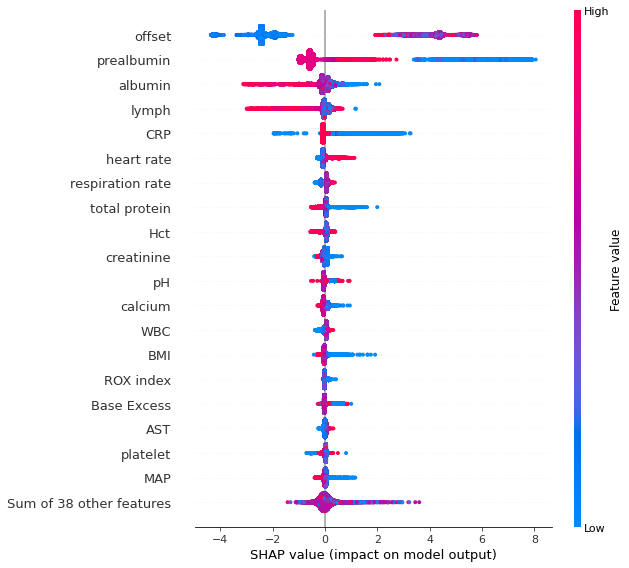
\includegraphics[width=0.9\linewidth]{../img/eicu_full_shap_beeswarm_20.png}
    \caption{完整模型中各变量的平均SHAP值比较}
    \label{figure:full-shap}
\end{figure}

根据预测结果比较,选择含$57$个输入变量的CatBoost模型为完整模型。%
计算完整模型中各变量的平均SHAP值,结果如图\ref{figure:full-shap}所示。%
此摘要图展示了各个变量对预测结果的影响情况分布。%
例如,ICU入住天数(offset)对结果影响明显,且ICU入住天数越长,发生ICU综合症的概率越大。

根据变量的平均SHAP值大小和数据获取的难易程度,选择了$15$个变量作为输入,%
建立更加易于使用的紧凑模型。使用默认超参数的紧凑模型平均AUC为$90.219\%$。%
通过贝叶斯优化超参数后,紧凑模型的平均AUC达到了$90.682\%$,同时平均准确率为$96.120\%$。%
虽然预测结果的得分略低于完整模型,但是紧凑模型明显在临床上更加可行、更加易用。

\subsection{性能分析}

\begin{figure}[htb]
    \centering
    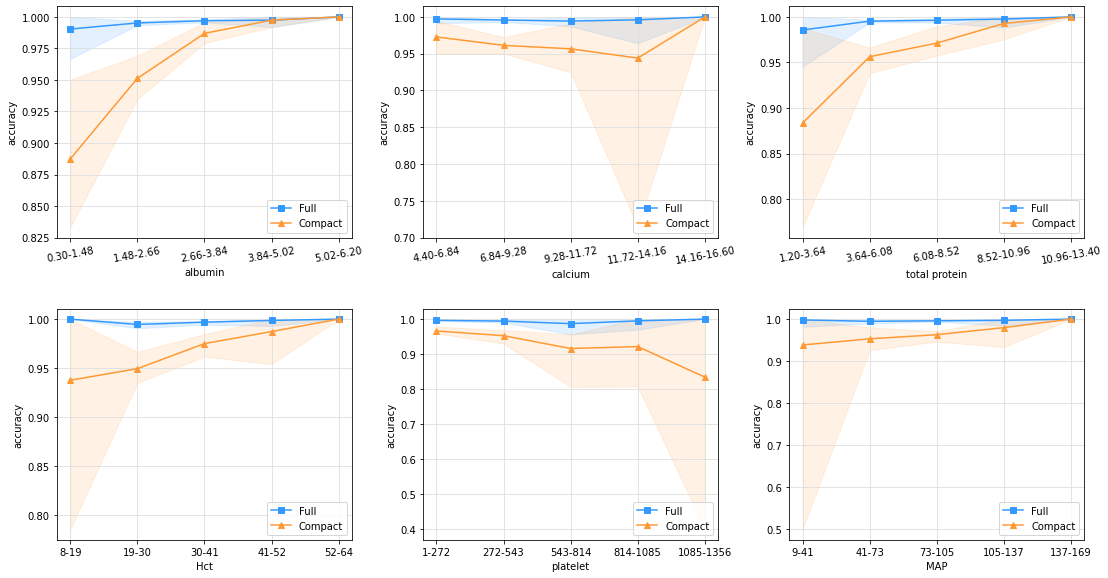
\includegraphics[width=\linewidth]{../img/eicu_performance.png}
    \caption{模型性能分析}
    \label{figure:model-performance}
\end{figure}

如图\ref{figure:model-performance}所示,完整模型和紧凑模型在各种指标的不同范围下都表现良好。%
当某个指标出现明显的异常值时,模型可以非常敏锐地察觉到并给出十分准确的预测结果。

\subsection{模型解释}

\begin{figure}[htb]
    \centering
    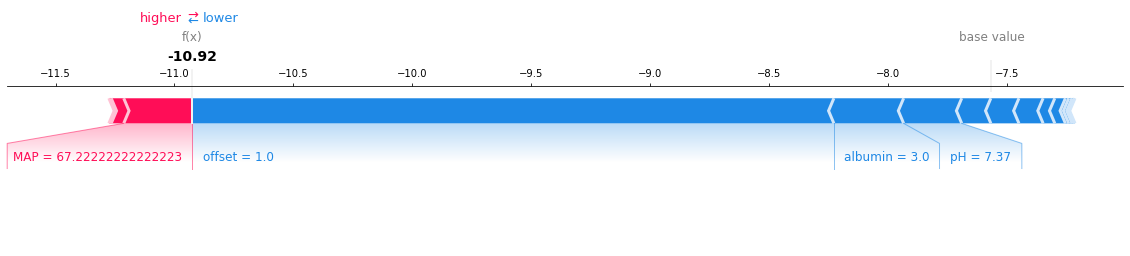
\includegraphics[width=\linewidth]{../img/eicu_compact_shap_force_neg.png}
    \vspace{-4em}
    \caption{个例(A)中主要变量的SHAP值}
    \label{figure:shap-neg}
\end{figure}

\begin{figure}[htb]
    \centering
    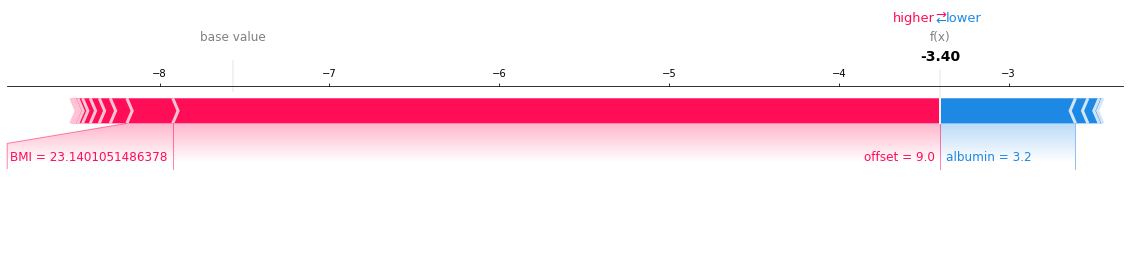
\includegraphics[width=\linewidth]{../img/eicu_compact_shap_force_pos.png}
    \vspace{-4em}
    \caption{个例(B)中主要变量的SHAP值}
    \label{figure:shap-pos}
\end{figure}

图\ref{figure:full-shap}从整体上展示了各个变量对于预测结果的影响情况,%
同时也展现了模型对输入变量变化的灵敏性。%
而图\ref{figure:shap-neg}和图\ref{figure:shap-pos}展示了两个个例中主要变量的SHAP值。%
图中红色条和蓝色条分别表示危险因素和安全因素,它们共同作用决定了最终的结果。%
如图\ref{figure:shap-neg},在个例(A)中,虽然患者的平均动脉压偏低,但是其ICU入住天数很短、%
血浆蛋白较多、pH值也良好,所以模型准确预测了患者次日无ICU综合症风险。%
又如图\ref{figure:shap-pos},在个例(B)中,虽然患者的血浆蛋白较多,%
但是其ICU入住天数较长、身体质量指数(BMI)偏低,所以模型准确预测了患者次日的ICU综合症。

\subsection{H5预测工具}

\newcommand\PredictionToolURL{http://1.15.185.22/sepsis-pics-tool/}

为了方便临床上对上述紧凑模型的测试,开发了一款预测脓毒症患者诱发ICU综合症的H5应用。%
只需在表单中输入指标数值,然后点击“提交”,就可以获得紧凑模型对患者次日发生ICU综合症概率的预测。%
目前应用已部署在此网址上:\url{\PredictionToolURL}。
